\documentclass[a4paper,man,floatsintext,natbib,donotrepeattitle]{apa6}

\usepackage[english]{babel}
\usepackage[utf8x]{inputenc}
\usepackage{amsmath}
\usepackage{graphicx}
\usepackage[colorinlistoftodos]{todonotes}
\usepackage{natbib}
\usepackage{subcaption}
\usepackage{pdfpages}
\usepackage{hyperref}
\usepackage{comment}

\hypersetup{
	colorlinks=true,
	linkcolor=black,
	citecolor=black,
	urlcolor=black
}

\definecolor{Blue}{RGB}{0,0,255}
\definecolor{Green}{RGB}{10,200,100}
\definecolor{Red}{RGB}{255,0,0}
\definecolor{Orange}{RGB}{255,140,0}
\definecolor{White}{RGB}{255,255,255}
\newcommand{\jd}[1]{\textcolor{Blue}{[jd: #1]}}  
\newcommand{\ek}[1]{\textcolor{Orange}{[ek: #1]}} 
\newcommand{\hideref}[1]{\textcolor{White}{[refs: #1]}} 

\newcommand{\subsubsubsection}[1]{{\em #1}}
\newcommand{\eref}[1]{(\ref{#1})}
\newcommand{\tableref}[1]{Table \ref{#1}}
\newcommand{\figref}[1]{Figure~\ref{#1}}
\newcommand{\appref}[1]{Appendix \ref{#1}}
\newcommand{\sectionref}[1]{Section \ref{#1}}

%\title{TITLE}
\shorttitle{INSERT SOME SHORT TITLE}
%\author{Elisa Kreiss} 
%\affiliation{Osnabrueck University}

\begin{document}

\pagenumbering{Roman}

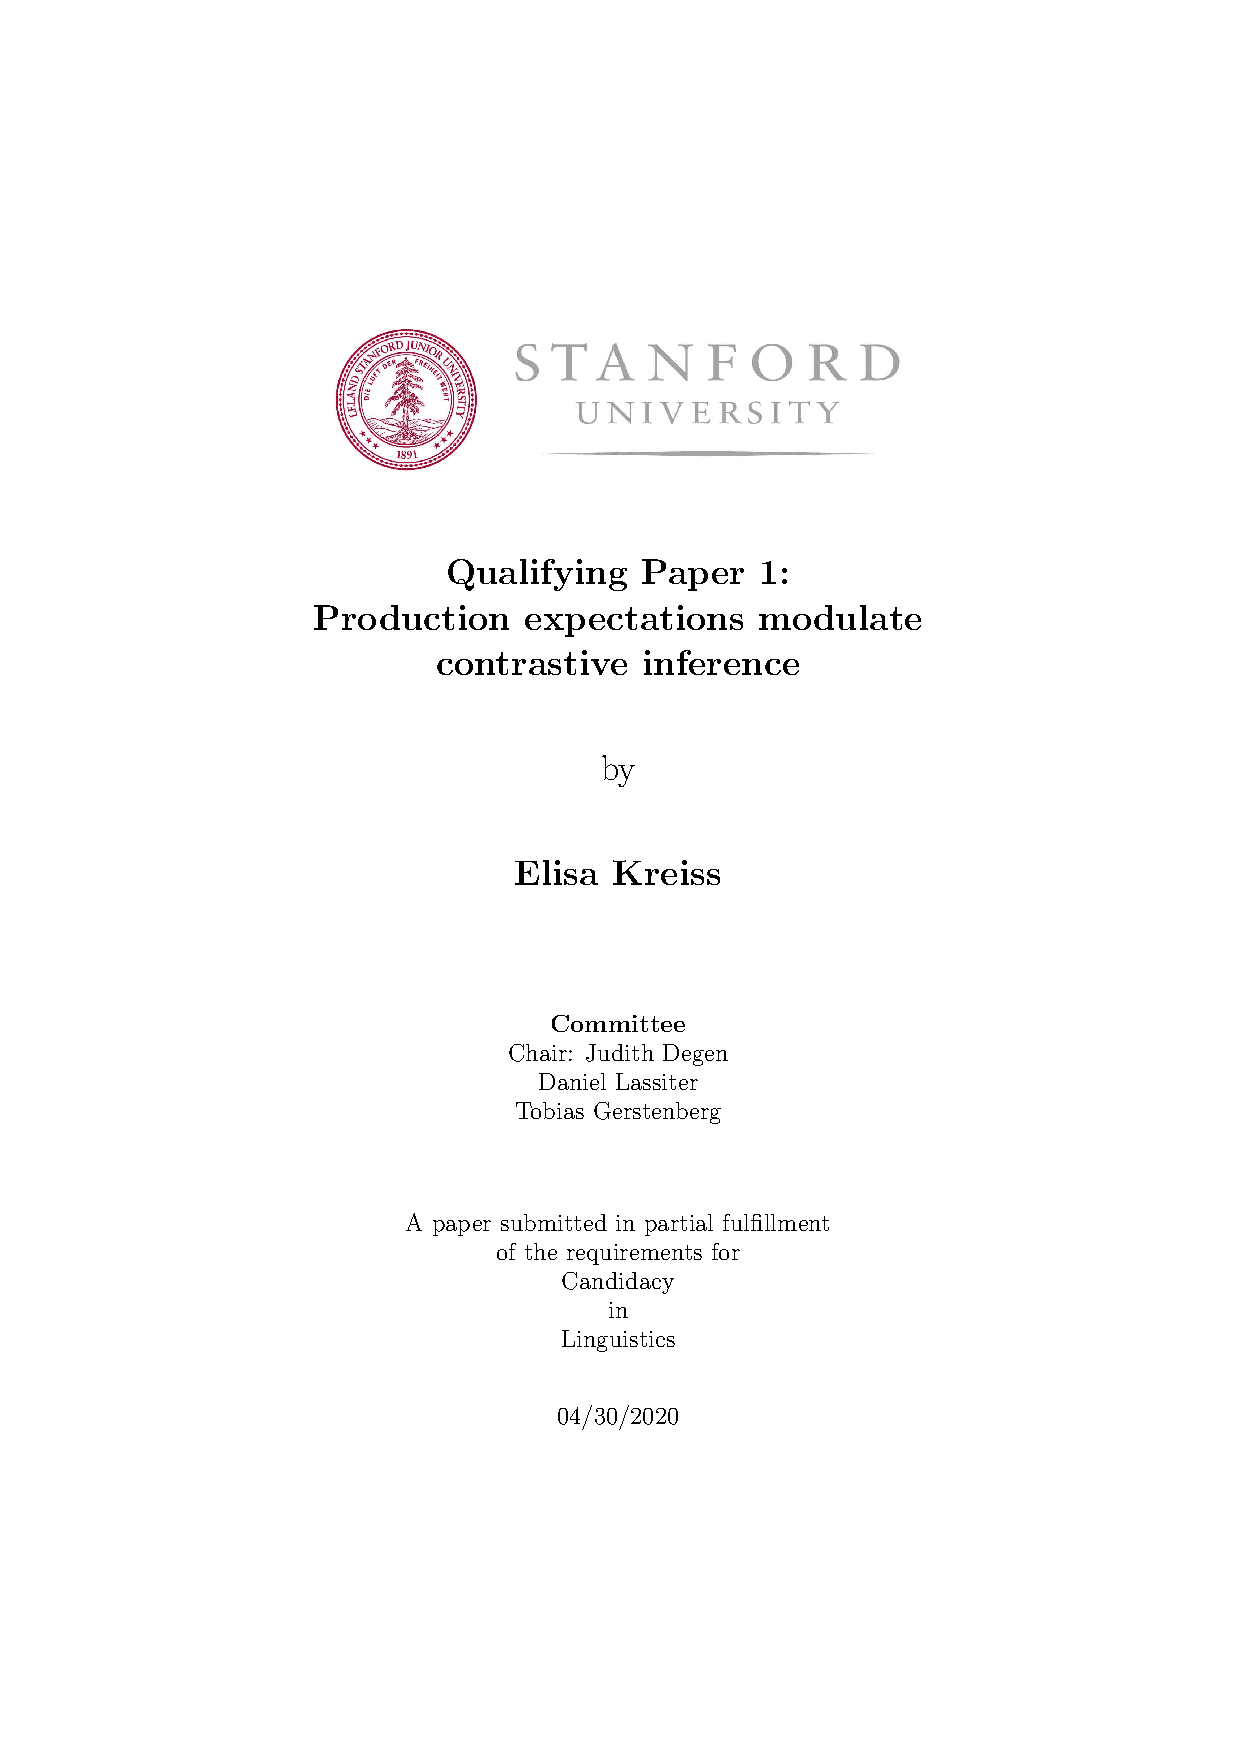
\includepdf[pages={1}]{titlepage/titlepage.pdf}

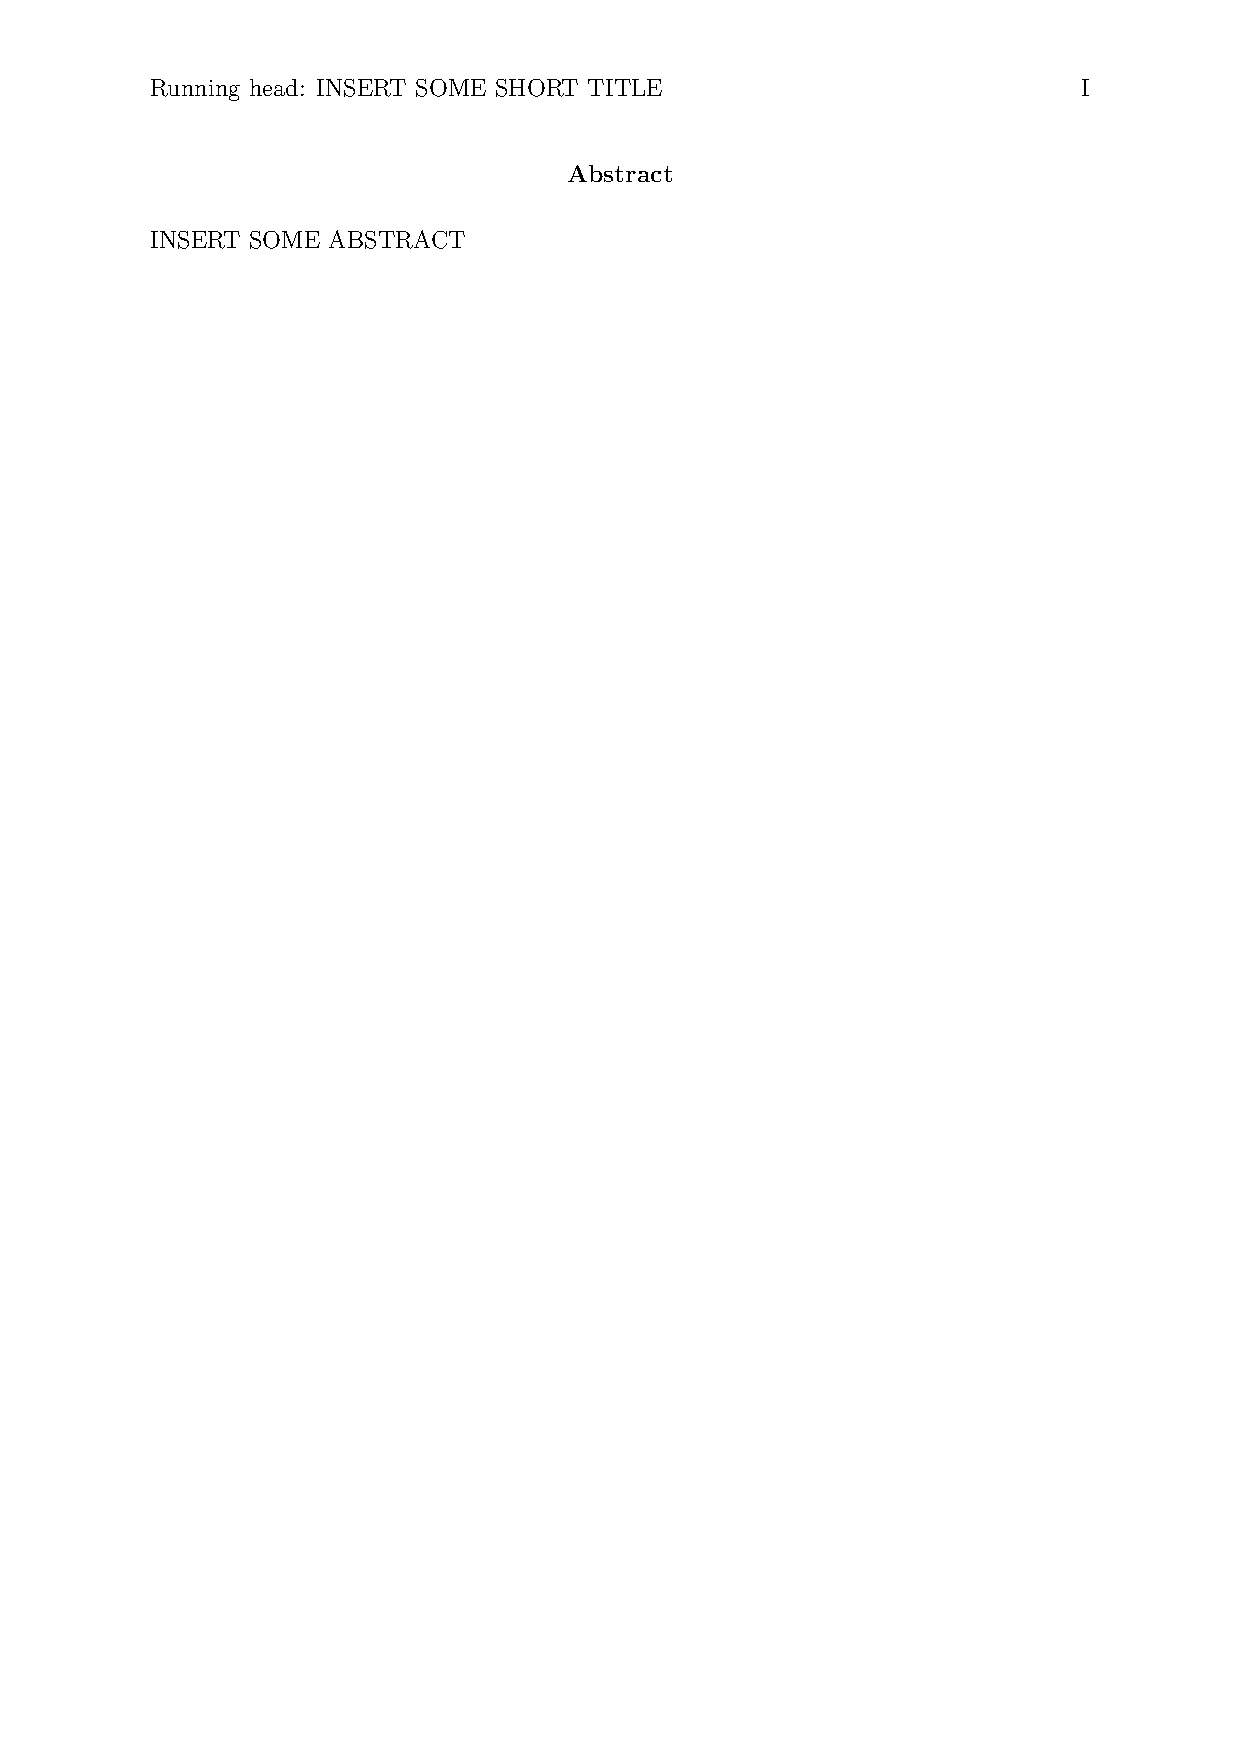
\includepdf[pages={1}]{abstract/abstract.pdf}

\clearpage

%{\def\addcontentsline#1#2#3{}}
\setcounter{page}{2}
\tableofcontents

\setcounter{secnumdepth}{3}

\clearpage

\ek{determine how to spell (non)colordiagnosticity}
\ek{watch your tenses; define a common textit/quotation style}

\pagenumbering{arabic}
\setcounter{page}{1}

% \section{Introduction}
% \subsection{SOME SUBSECTION}\label{sec:somesubsection}

\section{Experiment: Norming} \label{experiment}

We want to manipulate the modifier production probabilities a listener can expect from a speaker for an object in isolation. Color modifiers are more likely to be used in isolation (i.e., redundantly) than other adjective types \cite{Pechmann:1982}. Furthermore, their use is not arbitrary but dependent on the noun they modify \cite{Tanaka:1999,Sedivy:2003}. If one particular color is a defining property for the object, the object is \textit{color-diagnostic} and speakers rarely use the color modifier redundantly to refer to it \cite{Tanaka:1999}. Color-diagnostic objects are for example bananas, which are generally associated with the color yellow. Cups on the other hand are non-color-diagnostic objects, since they are not associated with one particular color and color itself is not a perceptual property that defines it. Even though a sportscar is primarily associated with the color red, color itself is not a defining perceptual property of the object, which is why it is also considered a non-color-diagnostic object \cite{Tanaka:1999}. 

Although color-diagnostic objects are rarely modified redundantly when they occur in their typical color, they often are when they occur in an atypical color instead. For example, a yellow banana is mainly referred to as \textit{a banana}, while a blue banana is referred to as \textit{a blue banana} \cite{Westerbeek:2015}. To manipulate the modifier production probabilities a listener can expect, we therefore use typical and atypical instances of color-diagnostic objects.

This design posits a number of requirements onto the items used in the study, which is why a variety of objects was carefully normed and then a subset of them was selected for the experiments. In addition to being color-diagnostic (Experiment \ref{coldiagnorming}), the items had to be shape-diagnostic, such that they would still be recognizable when changing their color. For example, plums, oranges and lemons can barely be told apart when changing their color to something atypical (Experiment \ref{freeprodnorming}). The items also have to be known to most participants and be easily recognizable (Experiment \ref{nameabilitynorming} and \ref{freeprodnorming}). Since participants will hear the utterance in the eye-tracking experiment, there should only be one potential label for the object to avoid surprisal artifacts at the noun onset \ek{citation?}.

Furthermore to our knowledge, previous experiments that manipulated the color typicality of objects, the colors used for typical and atypical instances of objects were not counterbalanced with respect to color, such that for example the color blue primarily occurred as an atypical instance while the color green occurred as a typical one. Since colors vary in their salience and affect eye movement \ek{cite!}, this imbalance might be a non-negligible confound to the typicality effect. Each color in our data set occurs twice as a typical instance and twice as an atypical instance.

Finally, the typical and atypical instance of each object was normed to ensure that the color manipulation of the images show the desired difference in typicality ratings (Experiment \ref{typicalitynorming}).

Motivated through our experimental design \ek{more?}, we aimed to find ten color diagnostic objects, evenly distributed over five different colors. To find the most ideal items, we started off with six colors (green, orange, pink, red, white, yellow), each with four possible typical color-diagnostic instances (24 items in total).

\subsection{Norming for color-diagnosticity}
\label{coldiagnorming}
% List feature norming

% Goal: determine color diagnosticity
% (1) Is color a property that is closely associated with the object?
% (2) If a color is mentioned, do participants agree on the color?

% Task: "List 3 perceptual features of a \textbf{NOUN}"

% free production and checkbox with possibility to say "I don't know this object."

% 52 trials;
% 4 control trials with nonce words;
% 25 presumably color diagnostic objects (4 for each of the 6 colors + 1 more green thing) and 23 presumably non-color diagnostic objects

% 40 participants;
% exclusion criteria: everyone correctly identified the 4 nonce words as unknown objects; and if they rated more than 8 objects as "object unknown" they were excluded (2 participants);
% resulting number of participants: 38

% we evaluated the results according to whether 
% (1) a color was mentioned at all in the features
% (2) a color was mentioned as a first feature
% (3) if a color was mentioned, was it the same or did they differ

Firstly, all potential stimuli were normed for their color-diagnosticity. Items are considered color-diagnostic if color is a perceptual property that is closely associated with the object, and if there is agreement on the specific color it is associated with \cite{Tanaka:1999}.

\paragraph{Participants}
We recruited 40 participants over Amazon's Mechanical Turk. \ek{add participant recruitment information/payment/duration/...} All participants indicated that their native language was English.

\paragraph{Materials and procedure}
The experimental design is adapted from \cite{Tanaka:1999}. 
Participants were asked to list three perceptual features of an object, which they entered into three free production text boxes. They could proceed to the next trial if they either entered all three features or indicated by a button press that they did not know the object. In the beginning of the experiment, participants saw an example trial where the term ``perceptual feature'' was defined and showed an example response for the object \textit{dime}, which was described as \textit{round}, \textit{shiny}, and \textit{small} (as used in \cite{Tanaka:1999}).
Each participant saw 52 trials, four of which were control trials with nonce words. From the remaining trials, 25 asked for presumably color-diagnostic objects (four for each of the six colors and one additional green object), and 23 asked for presumably non-color-diagnostic objects. \ek{Figure: show example design, possibly next to example trial}

\paragraph{Analysis and exclusions}
All participants indicated that they were unfamiliar with the four nonce words we included as attention checks. Two participants were excluded because they rated more than eight objects as unknown to them, resulting in a total of 38 participants.

\paragraph{Results}
We evaluated the results according to whether a color was mentioned as a first feature, and if a color was mentioned did participants agree on a specific color. The goal is to find five colors, each of which have two highly color-diagnostic objects.

First of all, color was more likely to be mentioned for the objects that were intended to be color-diagnostic and less likely for the non-color-diagnostic ones \ek{Figure}. An exception to that is bell pepper which is expected to be non-color-diagnostic but for which participants still mention color as an important perceptual feature. However bell pepper is not only associated with one specific color. Although it was mainly described as \textit{green}, several participants also mentioned \textit{red}. For all items that were intended to be color-diagnostic it holds that, if a color was mentioned, participants generally agreed on the color. 

Figure \ek{ref} shows the proportion of color mention as the first perceptual feature, facetted by the color they were associated with. The dashed horizontal line marks the case when color was mentioned half of the time as the first perceptual feature. The items in the colors pink and white have the lowest proportion of color mention overall, suggesting that most likely one of these colors will not be used for the final data set. Items will low proportions of color mention in each color are less likely to be chosen as stimuli. 


\subsection{Norming for nameability}
\label{nameabilitynorming}

% Goal: Are the image depictions we chose nameable, the way we intended?

% Task: "What is this?"

% free production

% 50 trials;
% 26 depictions of presumably color diagnostic objects (same as in color diagnosticity norming + 1 more lettuce depiction) and 24 presumably non-color diagnostic ones (same as in color diagnosticity norming + 1 more (sports)car);

% 20 participants;
% exclusion: 2 participants because they indicated that they were confused or didn't do the HIT correctly;
% resulting number of participants: 18

% We evaluated the results according to how many labels were used. If more than one label was used, we favored cohort competitors over entirely separate terms (e.g., bike and bicycle are more acceptable than traffic cone and cone);
% Wrt to lettuce we had romaine and iceberg lettuce depictions. The simple noun lettuce was more frequently used for the iceberg than the romaine lettuce which is why we favored the iceberg lettuce.; 
% other things: zucchini was half of the time misclassified as cucumber, similarly for pickle, traffic cone had a lot of different labels, such as simply cone, caution cone, hazard cone, safety cone

After we normed for color-diagnosticity, we chose image depictions of the items and normed them for their nameability. 

\paragraph{Participants}
We recruited 20 participants over Amazon's Mechanical Turk. \ek{add participant recruitment information/payment/duration/...} All participants indicated that their native language was English.

\paragraph{Materials and procedure}
Each participant saw 50 trials in which they were asked ``What is this?'' with a depiction of an object and a free production text field.
We used the same objects as in the color-diagnosticity norming study (i.e., 25 color-diagnostic objects and 23 non-color-diagnostic ones), but added an additional depiction for the lettuce and the sportscar.

\paragraph{Exclusions}
Two participants were excluded because they indicated that they were unsure whether they did the experiment correctly, resulting in a total of 18 participants.

\paragraph{Results}
We evaluated the results according to how many labels were used. If more than one label was used, we favored cohort competitors over entirely separate terms (e.g., \textit{bike} and \textit{bicycle} are more acceptable deviations than \textit{traffic cone} and \textit{cone}).

Overall, participants agreed on the label to give to the different objects. However there were also some problematic items. Both, the pickle and zucchini, were called cucumbers and for the zucchini this even happened to the same degree as the actual label. Given that they also have a low shape-diagnosticity, presenting them in atypical colors will most likely even worsen these issues, which is why they are candidates to exclude. Other items that received a variety of labels were the traffic cone (e.g., \textit{traffic cone, cone, caution cone, hazard cone}) and the rubber duck (e.g., \textit{rubber duck, duck, duck toy}). These cases are problematic because the different labels are not cohort competitors of each other, which will be relevant for the eyetracking experiments. 

Finally, we investigated which depiction represents the generic lettuce the best: romaine or iceberg. We found that when participants saw the iceberg lettuce before the romaine lettuce, they simply called it \textit{lettuce}. However, if they saw the romaine lettuce first, they called it \textit{romaine lettuce} 20\% of the time. This suggests that the iceberg lettuce is the more prototypical lettuce (in the MTurk community). 


\subsection{Norming for typicality}
\label{typicalitynorming}

% Goal: Does the color manipulation of the images show the desired difference in typicality ratings?

% Task: "How typical is this object for a \textbf{NOUN}?"

% slider rating, underlyingly coded as ranging from 0 to 100

% 45 trials;
% 11 color diagnostic objects, each in their typical color and 1-2 atypical colors (i.e., 25 stimuli); 20 non-color diagnostic stimuli

% 30 participants;
% exclusions: none; everyone thought they did the HIT correctly

% Results: generally clear distinction between typical and atypical instance;
% From the three items that were normed in two atypical colors (carrot, corn, pumpkin), we see the biggest difference between the red and white pumpkin. Therefore, we should choose the white pumpkin and (following from that) the green carrot and red corn.
% There does not seem to be a big difference between the yellow egg and snowman, but the white egg is rated even more typical and its size fits better to the other stimuli. Therefore, we should choose the egg over the snowman (given that both are also nameable).
% Even though the orange banana is predominantly rated below 50, it is still not as atypical as other objects.;
% The non-color diagnostic objects are all rated as very typical instances.

\paragraph{Participants}
We recruited 30 participants over Amazon's Mechanical Turk. \ek{add participant recruitment information/payment/duration/...} All participants indicated that their native language was English.

\paragraph{Materials and procedure}

\paragraph{Results}

\subsection{Norming for free production}
\label{freeprodnorming}

% Goal: Are the image depictions we chose nameable, the way we intended?

% Task: "What is this?"

% free production

% 31 trials (22 cd -- each participant saw one instance of each object at random, i.e., either typical or atypical; 20 non-cd)

% Results: swan is often called a goose; two people identified the white carrot as parsnip

% \subsection{Final stimuli selection}

% In the end, we have 10 objects, each occurring in a typical and atypical color.
% Items can occur in the colors yellow, red, green, orange and white. Each color occurs twice as typical and twice as atypical. This counterbalance aims to reduce artifacts of salience such as red is generally more salient as a warn signal \ek{ref?} and blue is highly atypical for most objects. A full list of stimuli can be found in table \ek{add table and reference}.

\subsection{Norming for multiple choice}


\subsection{Conclusion}


\section{Rational Speech-Act Model}

\bibliography{QP1}

\vfill
\pagebreak

\end{document}

%
% Please see the package documentation for more information
% on the APA6 document class:
%
% http://www.ctan.org/pkg/apa6
%





















% \section{Experiment: Comprehension} \label{experiment}

% \subsection{Method}

% \paragraph{Participants}
% We recruited 80 participants over Amazon's Mechanical Turk, 40 for each color competitor typicality manipulation. The study took on average 7 minutes and each of them were paid \ek{...} for their participation. We restricted participation to workers with IP addresses in the US and a approval rate of previous work above 97\%.

% \paragraph{Procedure}
% This experiment is a one-player adaptation of the production study explained in \ek{ref to section} and follows the design of an incremental decision task \ek{cite Qing}. participants were put into the listener role of the reference game. That means, they needed to identify which object was the target given a referring expression placed above the grid. Crucially, they do not observe the complete referring expression at once, but instead the utterance is gradually revealed. After new information is revealed, participants are required to make their best guess onto which object is the most likely target. The choices had to be made prior any disambiguating information (after observing "Click on the"), after observing an adjective ("Click on the yellow") and after observing the fully disambiguating noun ("Click on the yellow banana!"). The clicks before information are observed are useful to determine whether there are already strong priors in item selections, even before any information were observed. The clicks after revealing the adjective are the critical clicks that will affect our interpretation of inferences drawn from the adjective. After observing the noun there is only one possible referent left. These clicks are used as attention checks.

% Participants completed 55 trials in total, 20 of which were critical trials and 35 were fillers. The filler trials were supposed to ensure that participants perceive the referring expressions as being generated by a natural speaker. Firstly, all target trials are color modified utterances. To avoid that participants learn that the color modifier is always part of the referring expression, we need utterances that only have the bare noun. Second of all, we need to make sure that targets are not logically derivable. In a context such as \ek{Fig ref!}, the target can be determined by reasoning about the distractor choice. The target is the only object that shares the type (i.e., banana) with a distractor and its color (i.e., yellow) with another distractor. One can then derive that the object that is being distracted from will be the target. This regularity could also be learnt over the time course of the experiment. The filler trials therefore need to introduce primarily unmodified referring expressions that target other objects in the display. The exact trial structure is summarized in table \ref{tab:trialstructure}.

% \begin{table}[]
% 	\begin{tabular}{llll}
% 	\textbf{trial type} & \textbf{number} & \textbf{utterance} & \textbf{referent}           \\
% 	critical            & 20              & modified           & target                      \\
% 	filler              & 5               & unmodified         & color competitor (typical)  \\
% 	filler              & 5               & modified           & color competitor (atypical) \\
% 	filler              & 5               & modified           & contrast                    \\
% 	filler              & 20              & unmodified         & distractor (typical)       
% 	\end{tabular}
% 	\vspace{2mm}
% 	\caption{Overview of the trial structure for the comprehension study.}
% 	\label{tab:trialstructure}
% \end{table}

% Before participants proceeded to the main trials, they had to complete four practice trials constructed from the speaker perspective. In the speaker role, they saw a grid of four non-color diagnostic objects, one of which was marked as the target by a green border surrounding it. They were then asked to refer to the object such that a second player could identify it. The practice trials were introduced to familiarize the participants with the task.

% The main trials were randomized with one restriction: Trials in which we expect a color modifier to be superfluous or even misleading only occurred after the 15th trial. These were contexts where there was no contrast and either both target and color competitor typical objects, or the target typical while the color competitor was atypical. This measure should minimize the risk that participants perceive the "utterance generator" as unnatural.

% \paragraph{Materials}

% \ek{add choice of contexts (i.e., one per color,...); clarify what is within and between-subject manipulation with rationale}

% The stimuli were the same as in the production study.

% \paragraph{Data Preprocessing and exclusion}

% We excluded participants who indicated that they did the Hit incorrectly or were confused (7), who indicated that they had a native language other than English (4), who gave more then 20\% erroneous responses (2) and who did the Hit multiple times (1). Overall, we excluded 14 out of 80 submissions (17.5\%). An erroneous response is defined as a click to a non-target object after observing the fully disambiguating noun, i.e., participants are excluded who selected the wrong final object more than 11 times.

% \subsection{Results}

% \section{Discussion}